\documentclass[a4paper, 12pt]{article}
\usepackage[a4paper,top=1.5cm, bottom=1.5cm, left=1cm, right=1cm]{geometry}
\usepackage{cmap}					% поиск в PDF
\usepackage{mathtext} 				% русские буквы в формулах
\usepackage[T2A]{fontenc}			% кодировка
\usepackage[utf8]{inputenc}			% кодировка исходного текста
\usepackage[english,russian]{babel}	% локализация и переносы

\usepackage{amsmath,amssymb}
\usepackage{indentfirst}
\usepackage{longtable}
\usepackage{graphicx}
\usepackage{array}
\usepackage{float}

\usepackage{floatflt}
\usepackage{wrapfig}
\usepackage{siunitx} % Required for alignment
\usepackage{subfigure}
\usepackage{multirow}
\usepackage{rotating}
\usepackage{caption}

\graphicspath{{.}}


\title{\begin{center}Лабораторная работа №3.5.1\end{center}
Изучение плазмы газового разряда в неоне}
\author{Рожков А. В.}
\date{\today}

\begin{document}
    \pagenumbering{gobble}
    \maketitle
    \newpage
    \pagenumbering{arabic}

    \textbf{Цель работы}: изучение вольт-амперной характеристики тлеющего разряда, изучение свойств плазмы методом зондовых характеристик.


    \textbf{В работе используются}: стеклянная газоразрядная трубка, наполненная изотопом неона, высоковольтный источник питания (ВИП), источник питания постоянного тока, делитель напряжения, резистор, потенциометр, амперметры, вольтметры, переключатели.
    \section{Теория}

        \subsection*{Плазма}

            В ионизированном газе поле ионов <<экранируется>> электронами. Для поля $\mathbf{E}$ и плотности $\rho$ электрического заряда

            $$
                \text{div}~\mathbf{E} = 4 \pi \rho,
            $$

            а с учётом сферической симметрии и $\mathbf{E} = -\text{grad}~\varphi$:

            \begin{equation}
                \dfrac{d^2 \varphi}{dr^2}+\dfrac{2}{r}\dfrac{d\varphi}{dr}=-4\pi \rho.
            \end{equation}

            Плотности заряда электронов и ионов (которые мы считаем бесконечно тяжёлыми и поэтому неподвижными)
            \begin{equation}
                \begin{array}{c}
                    \rho_e = -ne \cdot \exp\left(\dfrac{e\varphi}{kT_e}\right),\\
                    \rho_i = ne.
                \end{array}
            \end{equation}

            Тогда из $(1)$ в предположении $\dfrac{e\varphi}{kT_e} \ll 1$ получим

            \begin{equation}
                \varphi = \dfrac{Ze}{r}e^{-r/r_D},
            \end{equation}

            где $r_D = \sqrt{\dfrac{kT_e}{4\pi n e^2}}$ -- \textit{радиус Дебая}. Среднее число ионов в сфере такого радиуса

            \begin{wrapfigure}{r}{4cm}
                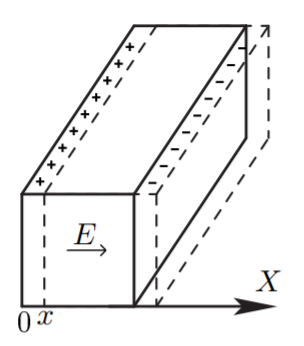
\includegraphics[scale=0.5]{img/2.png}
            \end{wrapfigure}

            \begin{equation}
                N_D = n\dfrac{4}{3}\pi r_D^2.
            \end{equation}

            Теперь выделим параллелепипед с плотностью $n$ электронов, сместим их на $x$. Возникнут поверхностные заряды $\sigma = nex$, поле от которых будет придавать электронам ускорение:

            $$
                \dfrac{d^2x}{dt^2}=-\dfrac{eE}{m}=-\dfrac{4\pi n e^2}{m}x.
            $$

            Отсюда получаем \textit{плазменную (ленгмюровскую) частоту} колебаний электронов:

            \begin{equation}
                \omega_p = \sqrt{\dfrac{4\pi ne^2}{m}}.
            \end{equation}

        \subsection*{Одиночный зонд}

            При внесении в плазму уединённого проводника -- \textit{зонда} -- с потенциалом, изначально равным потенциалу точки плазмы, в которую его помещают, на него поступают токи электронов и ионов:

            \begin{equation}
                \begin{array}{c}
                    I_{e0} = \dfrac{n \langle v_e \rangle}{4}eS,\\
                    I_{i0} = \dfrac{n \langle v_i \rangle}{4}eS,
                \end{array}
            \end{equation}

            где $\langle v_e \rangle$ и $\langle v_i \rangle$ -- средние скорости электронов и ионов, $S$ -- площадь зонда, $n$ -- плотность электронов и ионов. Скорости электронов много больше скорости ионов, поэтому $I_{i0} \ll I_{e0}$. Зонд будет заряжаться до некоторого равновесного напряжения $-U_f$ -- \textit{плавающего потенциала}.

            \begin{wrapfigure}{r}{5.5cm}
                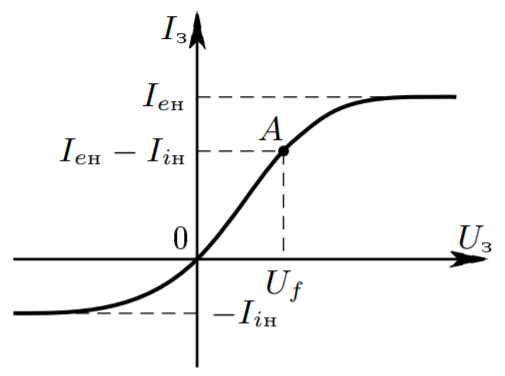
\includegraphics[scale=0.5]{img/3.png}
            \end{wrapfigure}

            В равновесии ионный ток мало меняется, а электронный имеет вид

            $$
                I_e = I_0 \exp\left( -\dfrac{eU_f}{kT_e} \right).
            $$

            Будем подавать потенциал $U_\text{з}$ на зонд и снимать значение зондового тока $I_\text{з}$. Максимальное значение тока $I_{e\text{н}}$ -- электронный ток насыщения, а минимальное $I_{i\text{н}}$ -- ионный ток насыщения. Значение из эмпирической формулы Бомона:

            \begin{equation}
                I_{i\text{н}} = 0.4 neS \sqrt{\dfrac{2kT_e}{m_i}}.
            \end{equation}

        \subsection*{Двойной зонд}

            Двойной зонд -- система из двух одинаковых зондов, расположенных на небольшом расстоянии друг от друга, между которыми создаётся разность потенциалов, меньшая $U_f$. Рассчитаем ток между ними вблизи $I=0$. При небольших разностях потенциалов ионные токи на оба зонда близки к току насыщения и компенсируют друг друга, а значит величина результирующего тока полностью связана с разностью электронных токов. Пусть потенциалы на зондах

            $$
                U_1 = -U_f + \Delta U_1,
            $$

            $$
                U_2 = -U_f + \Delta U_2.
            $$

            Между зондами $U = U_2 - U_1 = \Delta U_2 - \Delta U_1$.

            Через первый электрод

            \begin{equation}
                I_1 = I_{i\text{н}} + I_{e1} = I_{i\text{н}} - \dfrac{1}{4}neS\langle v_e\rangle \exp\left(-\dfrac{eU_f}{kT_e}\right)\exp\left(\dfrac{e\Delta U_1}{kT_e}\right)=I_{i\text{н}}\left(1 - \exp\left( \dfrac{e\Delta U_1}{kT_e} \right)\right).
            \end{equation}

            Аналогично через второй получим

            \begin{equation}
                I_2 = I_{i\text{н}}\left(1 - \exp\left( \dfrac{e\Delta U_2}{kT_e} \right)\right)
            \end{equation}

            Из $(7)$ и $(8)$ с учётом последовательного соединение зондов ($I_1 = -I_2 = I)$:

            $$
                \Delta U_1= \dfrac{kT_e}{e}\text{ln}\left(1 - \dfrac{I}{I_{i\text{н}}}\right)
            $$

            $$
                \Delta U_2= \dfrac{kT_e}{e}\text{ln}\left(1 + \dfrac{I}{I_{i\text{н}}}\right)
            $$

            Тогда итоговые формулы для разности потенциалов и тока

            \begin{equation}
                U = \dfrac{kT_e}{e}\text{ln}\dfrac{1 - I/I_{i\text{н}}}{1 + I/I_{i\text{н}}},
                I = I_{i\text{н}} \text{th}\dfrac{eU}{2kT_e}.
            \end{equation}

            Реальная зависимость выглядит несколько иначе и описывается формулой

            \begin{floatingfigure}[r]{0.3\textwidth}
                \centering
                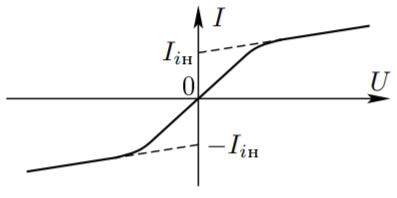
\includegraphics[width=0.3\textwidth]{img/4.png}
            \end{floatingfigure}

            \begin{equation}
                I = I_{i\text{н}} \text{th}\dfrac{eU}{2kT_e} + AU.
            \end{equation}

            Из этой формулы можно найти формулу для $T_e$: для $U=0$ мы найдём $I_{i\text{н}}$, продифференцируем в точке $U=0$ и с учётом $\text{th}~\alpha \approx \alpha$ при малых $\alpha$ и $A\rightarrow 0$ получим:

            \begin{equation}
                kT_e = \dfrac{1}{2}\dfrac{eI_{i\text{н}}}{\dfrac{dI}{dU}|_{U=0}}.
            \end{equation}

    \section{Описание установки}

        \begin{figure}[!ht]
            \centering
            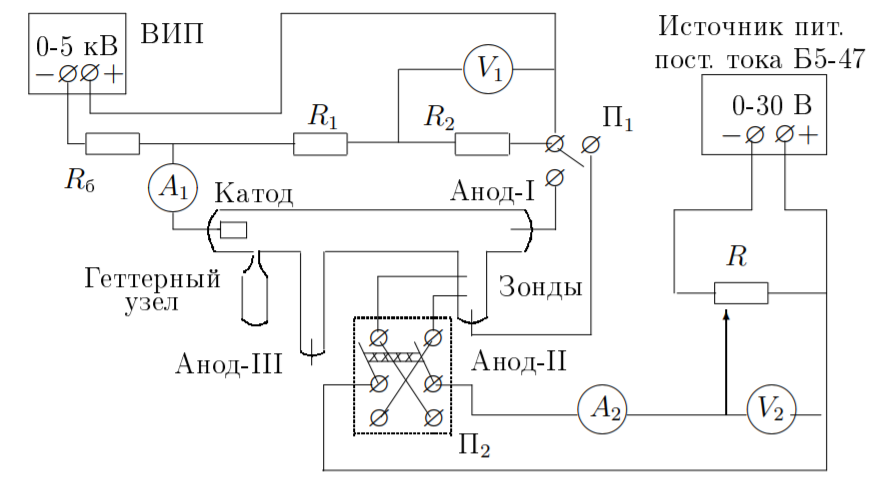
\includegraphics[width=0.6\textwidth]{img/1.png}
        \end{figure}

        Стеклянная газоразрядная трубка имеет холодный (ненакаливаемый) полый катод, три анода и \textit{геттерный} узел -- стеклянный баллон, на внутреннюю поверхность которого напылена газопоглощающая плёнка (\textit{геттер}). Трубка наполнена изотопом неона $^22$Ne при давлении 2 мм рт. ст. Катод и один из анодом (I и II) с помощью переключателя $\Pi_1$ подключается через балластный резистор $R_\text{б}$ ($\approx 450$ кОм) к регулируемому ВИП с выходным напряжением до 5 кВ.

        При подключении к ВИП анода-I между ним и катодом возникает газовый разряд. Ток разряда измеряется миллиамперметром $A_1$, а падение напряжения на разрядной трубке -- цифровым вольтметром $V_1$, подключённым к трубке через высокоомный (25 МОм) делитель напряжения с коэффициентом $(R_1+R_2)/R_2 = 10$.

        При подключении к ВИП анода-II разряд возникает в пространстве между катодом и анодом-II, где находятся двойной зонд, используемый для диагностики плазмы положительного столба. Зонды изготовлены из молибденовой проволоки диаметром $d = 0.2$ мм и имеют длину $l = 5.2$ мм. Они подключены к источнику питания GPS через потенциометр $R$. Переключатель $\Pi_2$ позволяет изменять полярность напряжения на зондах. Величина напряжения на зондах изменяется с помощью дискретного переключателя <<$V$>> выходного напряжения источника питания и потенциометра $R$, а измеряется цифровым вольтметром $V_2$. Для измерения зондового тока используется мультиметр $A_2$.

    \section{Ход работы}

        \subsection{ВАХ разряда}

            Построим ВАХ разряда

            \begin{figure}[!ht]
                \centering
                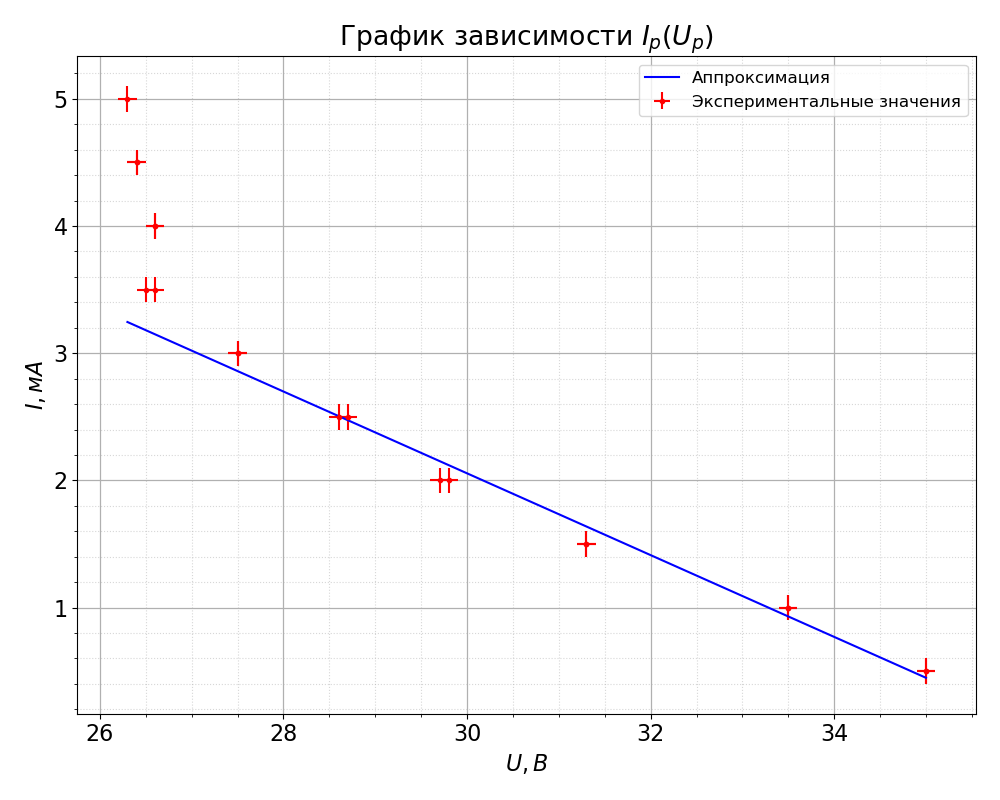
\includegraphics[width=0.75\textwidth]{img/vah_plazma.png}
                \caption{ВАХ разряда $I_p(U_p)$}
                \label{plot:vah_plazma}
            \end{figure}

            $$
                R_{диф} = \frac{dU}{dI} = (-3.06 \pm 0.12)~кОм
            $$

            Как видим по рисунку \ref{img:vah_plazma_labnik}, наш график соответствует участку ДГ - поднормальному тлеющему разряду.

            \begin{figure}[!ht]
                \centering
                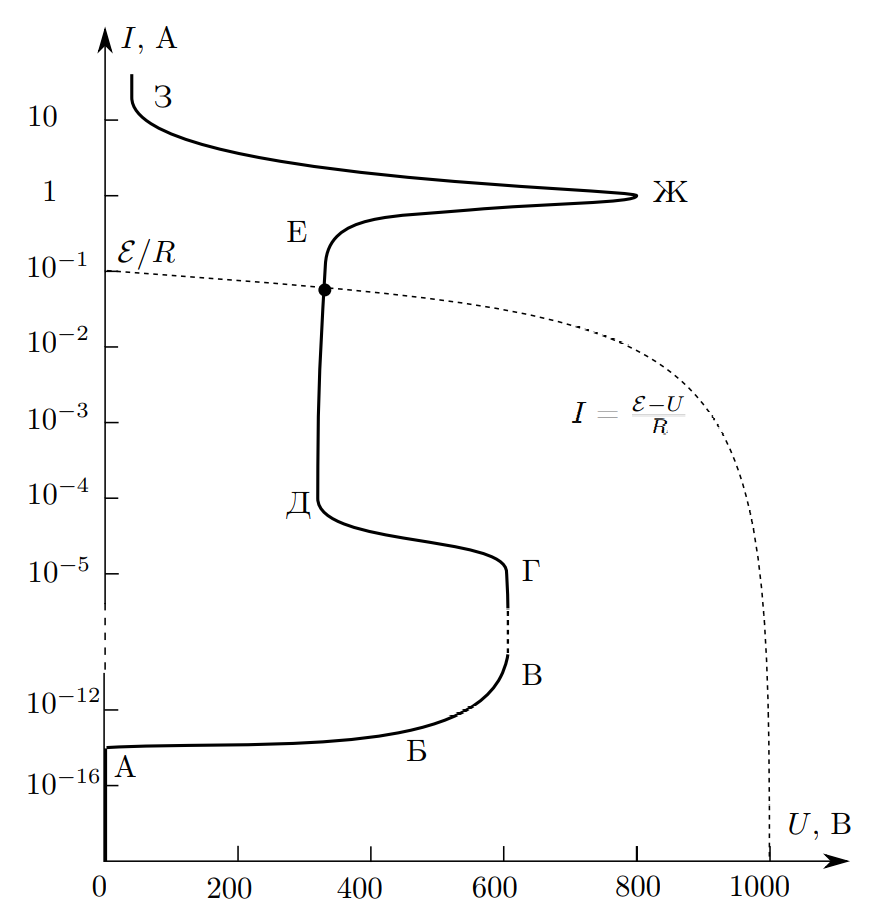
\includegraphics[width=0.5\textwidth]{img/5.png}
                \caption{ВАХ разряда}
                \label{img:vah_plazma_labnik}
            \end{figure}

        \subsection{Зондовые характеристики}

            Построим ВАХ зондов для различных значений тока разряда. На графиках представлены отцентрированные по вертикали значения. Также проведены асимптоты

            \begin{figure}[!ht]
                \centering
                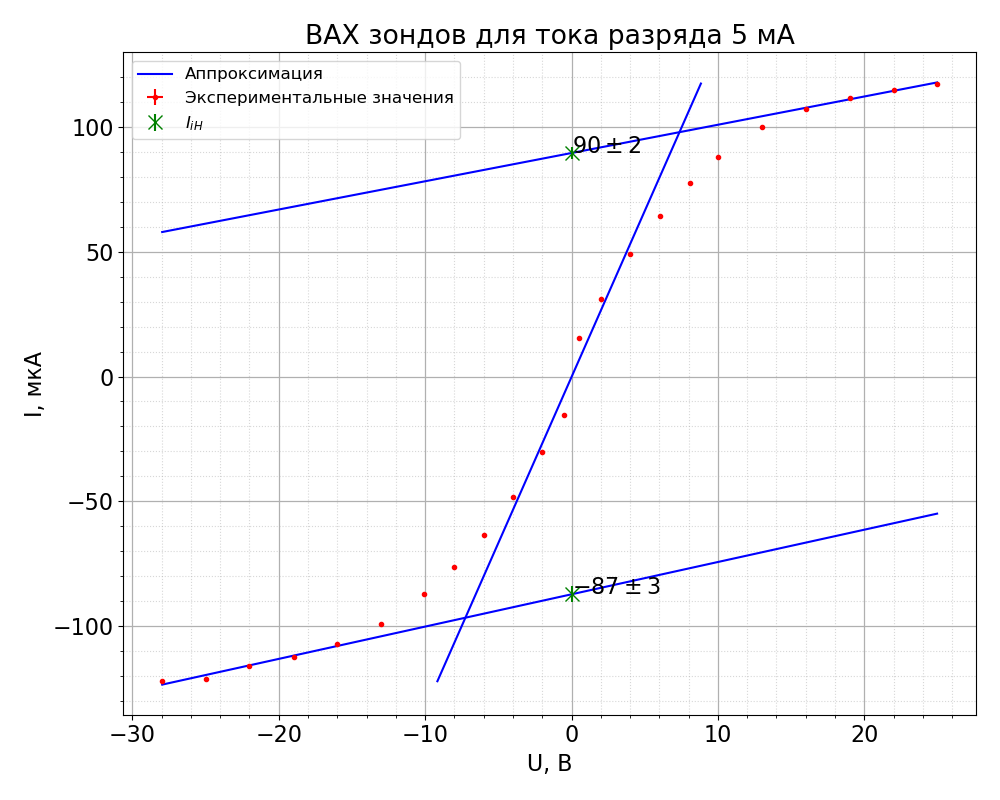
\includegraphics[width=0.6\textwidth]{img/vah_zond_5ma.png}
                \caption{ВАХ зонда $I(U) при токе разряда 5 мА$}
                \label{plot:vah_zond_5ma}
            \end{figure}

            \begin{figure}[!ht]
                \centering
                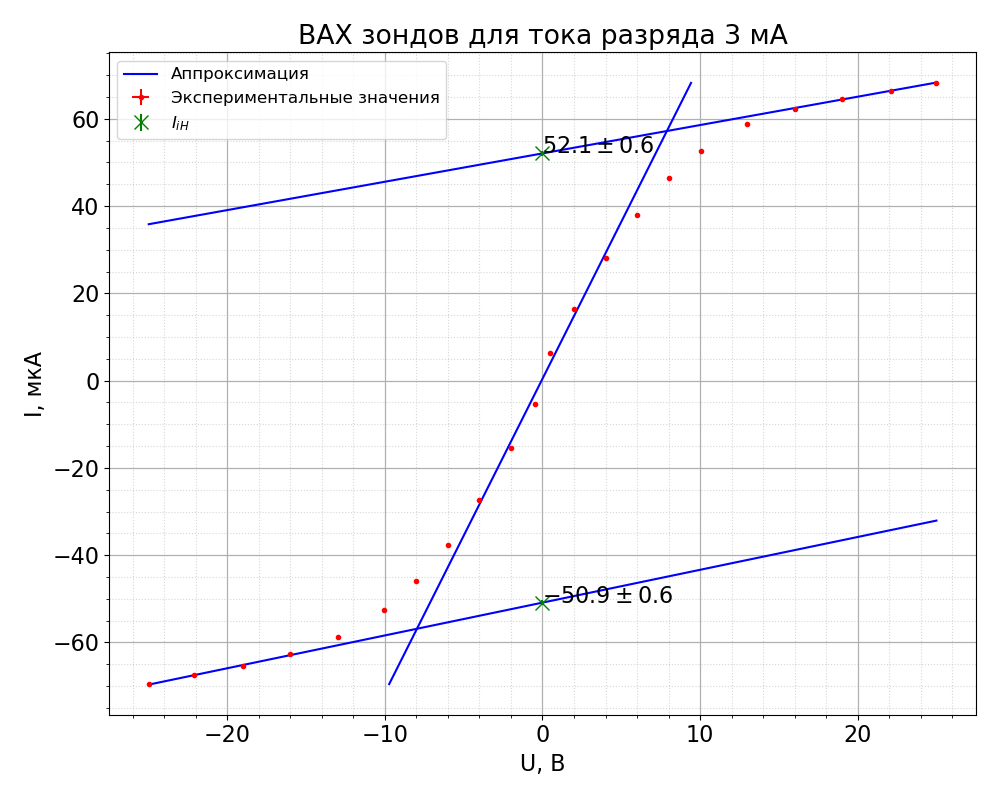
\includegraphics[width=0.6\textwidth]{img/vah_zond_3ma.png}
                \caption{ВАХ зонда $I(U) при токе разряда 3 мА$}
                \label{plot:vah_zond_3ma}
            \end{figure}

            \begin{figure}[!ht]
                \centering
                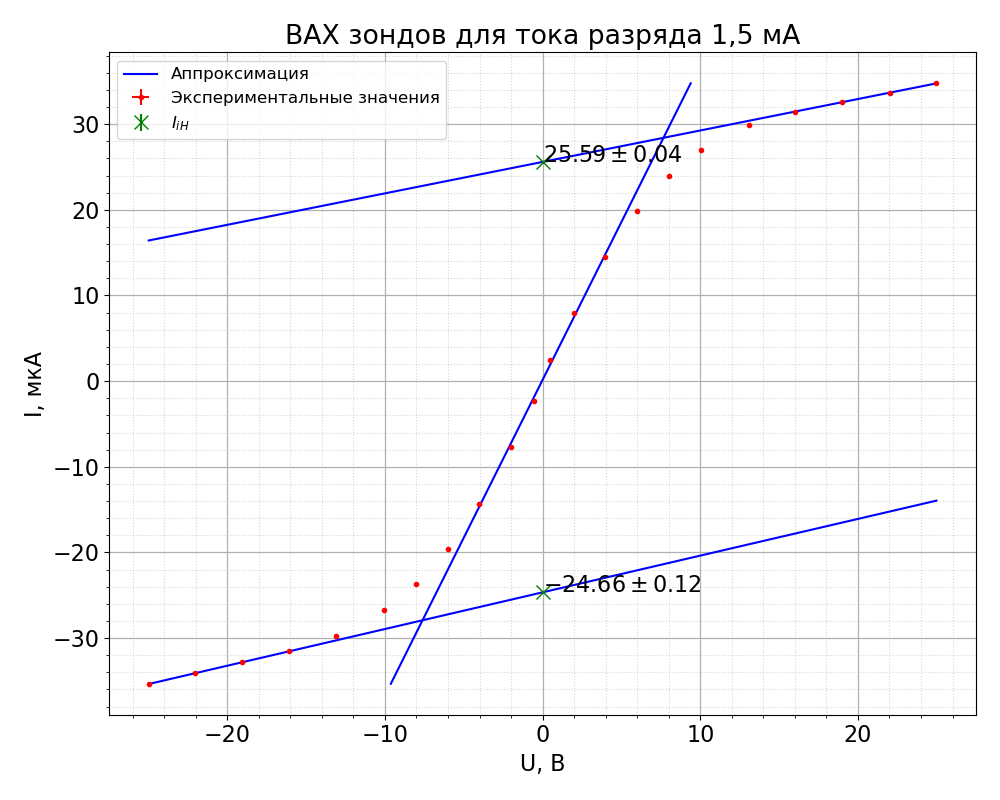
\includegraphics[width=0.6\textwidth]{img/vah_zond_15ma.png}
                \caption{ВАХ зонда $I(U) при токе разряда 1.5 мА$}
                \label{plot:vah_zond_15ma}
            \end{figure}

            Из точек пересечения асимптот с осью $U = 0$ найдём $I_{iH}$. Также определим $\frac{dI}{dU}$ в окрестности точки $U = 0$. При помощи этого рассчитаем температуру электронов.

            $$
                T_e = \frac{1}{2} \frac{e I_{iH}}{k \frac{dI}{dU} \vert_{U_0=0}}
            $$



\end{document}
